% GNUPLOT: LaTeX picture with Postscript
\begingroup
  \makeatletter
  \providecommand\color[2][]{%
    \GenericError{(gnuplot) \space\space\space\@spaces}{%
      Package color not loaded in conjunction with
      terminal option `colourtext'%
    }{See the gnuplot documentation for explanation.%
    }{Either use 'blacktext' in gnuplot or load the package
      color.sty in LaTeX.}%
    \renewcommand\color[2][]{}%
  }%
  \providecommand\includegraphics[2][]{%
    \GenericError{(gnuplot) \space\space\space\@spaces}{%
      Package graphicx or graphics not loaded%
    }{See the gnuplot documentation for explanation.%
    }{The gnuplot epslatex terminal needs graphicx.sty or graphics.sty.}%
    \renewcommand\includegraphics[2][]{}%
  }%
  \providecommand\rotatebox[2]{#2}%
  \@ifundefined{ifGPcolor}{%
    \newif\ifGPcolor
    \GPcolortrue
  }{}%
  \@ifundefined{ifGPblacktext}{%
    \newif\ifGPblacktext
    \GPblacktextfalse
  }{}%
  % define a \g@addto@macro without @ in the name:
  \let\gplgaddtomacro\g@addto@macro
  % define empty templates for all commands taking text:
  \gdef\gplbacktext{}%
  \gdef\gplfronttext{}%
  \makeatother
  \ifGPblacktext
    % no textcolor at all
    \def\colorrgb#1{}%
    \def\colorgray#1{}%
  \else
    % gray or color?
    \ifGPcolor
      \def\colorrgb#1{\color[rgb]{#1}}%
      \def\colorgray#1{\color[gray]{#1}}%
      \expandafter\def\csname LTw\endcsname{\color{white}}%
      \expandafter\def\csname LTb\endcsname{\color{black}}%
      \expandafter\def\csname LTa\endcsname{\color{black}}%
      \expandafter\def\csname LT0\endcsname{\color[rgb]{1,0,0}}%
      \expandafter\def\csname LT1\endcsname{\color[rgb]{0,1,0}}%
      \expandafter\def\csname LT2\endcsname{\color[rgb]{0,0,1}}%
      \expandafter\def\csname LT3\endcsname{\color[rgb]{1,0,1}}%
      \expandafter\def\csname LT4\endcsname{\color[rgb]{0,1,1}}%
      \expandafter\def\csname LT5\endcsname{\color[rgb]{1,1,0}}%
      \expandafter\def\csname LT6\endcsname{\color[rgb]{0,0,0}}%
      \expandafter\def\csname LT7\endcsname{\color[rgb]{1,0.3,0}}%
      \expandafter\def\csname LT8\endcsname{\color[rgb]{0.5,0.5,0.5}}%
    \else
      % gray
      \def\colorrgb#1{\color{black}}%
      \def\colorgray#1{\color[gray]{#1}}%
      \expandafter\def\csname LTw\endcsname{\color{white}}%
      \expandafter\def\csname LTb\endcsname{\color{black}}%
      \expandafter\def\csname LTa\endcsname{\color{black}}%
      \expandafter\def\csname LT0\endcsname{\color{black}}%
      \expandafter\def\csname LT1\endcsname{\color{black}}%
      \expandafter\def\csname LT2\endcsname{\color{black}}%
      \expandafter\def\csname LT3\endcsname{\color{black}}%
      \expandafter\def\csname LT4\endcsname{\color{black}}%
      \expandafter\def\csname LT5\endcsname{\color{black}}%
      \expandafter\def\csname LT6\endcsname{\color{black}}%
      \expandafter\def\csname LT7\endcsname{\color{black}}%
      \expandafter\def\csname LT8\endcsname{\color{black}}%
    \fi
  \fi
  \setlength{\unitlength}{0.0500bp}%
  \begin{picture}(11338.00,10204.00)%
    \gplgaddtomacro\gplbacktext{%
      \csname LTb\endcsname%
      \put(946,5840){\makebox(0,0)[r]{\strut{}-2}}%
      \put(946,6364){\makebox(0,0)[r]{\strut{}-1.8}}%
      \put(946,6888){\makebox(0,0)[r]{\strut{}-1.6}}%
      \put(946,7412){\makebox(0,0)[r]{\strut{}-1.4}}%
      \put(946,7937){\makebox(0,0)[r]{\strut{}-1.2}}%
      \put(946,8461){\makebox(0,0)[r]{\strut{}-1}}%
      \put(946,8985){\makebox(0,0)[r]{\strut{}-0.8}}%
      \put(946,9509){\makebox(0,0)[r]{\strut{}-0.6}}%
      \put(1078,5620){\makebox(0,0){\strut{}-0.8}}%
      \put(1602,5620){\makebox(0,0){\strut{}-0.6}}%
      \put(2127,5620){\makebox(0,0){\strut{}-0.4}}%
      \put(2651,5620){\makebox(0,0){\strut{}-0.2}}%
      \put(3175,5620){\makebox(0,0){\strut{} 0}}%
      \put(3699,5620){\makebox(0,0){\strut{} 0.2}}%
      \put(4224,5620){\makebox(0,0){\strut{} 0.4}}%
      \put(4748,5620){\makebox(0,0){\strut{} 0.6}}%
      \put(5272,5620){\makebox(0,0){\strut{} 0.8}}%
      \put(176,7674){\rotatebox{-270}{\makebox(0,0){\strut{}Position $y$ [$\si{\metre}$]}}}%
      \put(3175,5290){\makebox(0,0){\strut{}Position $x$ [$\si{\metre}$]}}%
      \put(3175,9839){\makebox(0,0){\strut{}Trajektorie}}%
    }%
    \gplgaddtomacro\gplfronttext{%
      \csname LTb\endcsname%
      \put(4285,9336){\makebox(0,0)[r]{\strut{}$m_1$}}%
      \csname LTb\endcsname%
      \put(4285,9116){\makebox(0,0)[r]{\strut{}$m_2$}}%
    }%
    \gplgaddtomacro\gplbacktext{%
      \csname LTb\endcsname%
      \put(6351,5806){\makebox(0,0)[r]{\strut{}-4}}%
      \put(6351,6273){\makebox(0,0)[r]{\strut{}-3}}%
      \put(6351,6740){\makebox(0,0)[r]{\strut{}-2}}%
      \put(6351,7207){\makebox(0,0)[r]{\strut{}-1}}%
      \put(6351,7675){\makebox(0,0)[r]{\strut{} 0}}%
      \put(6351,8142){\makebox(0,0)[r]{\strut{} 1}}%
      \put(6351,8609){\makebox(0,0)[r]{\strut{} 2}}%
      \put(6351,9076){\makebox(0,0)[r]{\strut{} 3}}%
      \put(6351,9543){\makebox(0,0)[r]{\strut{} 4}}%
      \put(6483,5586){\makebox(0,0){\strut{}-1.5}}%
      \put(7226,5586){\makebox(0,0){\strut{}-1}}%
      \put(7969,5586){\makebox(0,0){\strut{}-0.5}}%
      \put(8712,5586){\makebox(0,0){\strut{} 0}}%
      \put(9455,5586){\makebox(0,0){\strut{} 0.5}}%
      \put(10198,5586){\makebox(0,0){\strut{} 1}}%
      \put(10941,5586){\makebox(0,0){\strut{} 1.5}}%
      \put(5845,7674){\rotatebox{-270}{\makebox(0,0){\strut{}verallgemeinerter Impuls $p_{\theta}$ [$\si{\kilogram\metre\squared\per\second}$]}}}%
      \put(8712,5256){\makebox(0,0){\strut{}Auslenkung $\theta$ [$\si{\radian}$]}}%
      \put(8712,9873){\makebox(0,0){\strut{}Phasenraum}}%
    }%
    \gplgaddtomacro\gplfronttext{%
      \csname LTb\endcsname%
      \put(9954,9370){\makebox(0,0)[r]{\strut{}$\theta_1$}}%
      \csname LTb\endcsname%
      \put(9954,9150){\makebox(0,0)[r]{\strut{}$\theta_2$}}%
    }%
    \gplgaddtomacro\gplbacktext{%
      \csname LTb\endcsname%
      \put(946,704){\makebox(0,0)[r]{\strut{} 0.1}}%
      \put(946,1950){\makebox(0,0)[r]{\strut{} 1}}%
      \put(946,3196){\makebox(0,0)[r]{\strut{} 10}}%
      \put(946,4442){\makebox(0,0)[r]{\strut{} 100}}%
      \put(1078,484){\makebox(0,0){\strut{} 0}}%
      \put(2311,484){\makebox(0,0){\strut{} 5}}%
      \put(3544,484){\makebox(0,0){\strut{} 10}}%
      \put(4777,484){\makebox(0,0){\strut{} 15}}%
      \put(6010,484){\makebox(0,0){\strut{} 20}}%
      \put(7242,484){\makebox(0,0){\strut{} 25}}%
      \put(8475,484){\makebox(0,0){\strut{} 30}}%
      \put(9708,484){\makebox(0,0){\strut{} 35}}%
      \put(10941,484){\makebox(0,0){\strut{} 40}}%
      \put(176,2573){\rotatebox{-270}{\makebox(0,0){\strut{}Fourierkoeffizient $|g_k|$ [$\si{\radian}$]}}}%
      \put(6009,154){\makebox(0,0){\strut{}Kreisfrequenz $\omega$ [$\si{\radian\per\second}$]}}%
      \put(6009,4772){\makebox(0,0){\strut{}Leistungsspektrum von $\theta$}}%
    }%
    \gplgaddtomacro\gplfronttext{%
      \csname LTb\endcsname%
      \put(9954,4269){\makebox(0,0)[r]{\strut{}$\theta_1$}}%
      \csname LTb\endcsname%
      \put(9954,4049){\makebox(0,0)[r]{\strut{}$\theta_2$}}%
    }%
    \gplbacktext
    \put(0,0){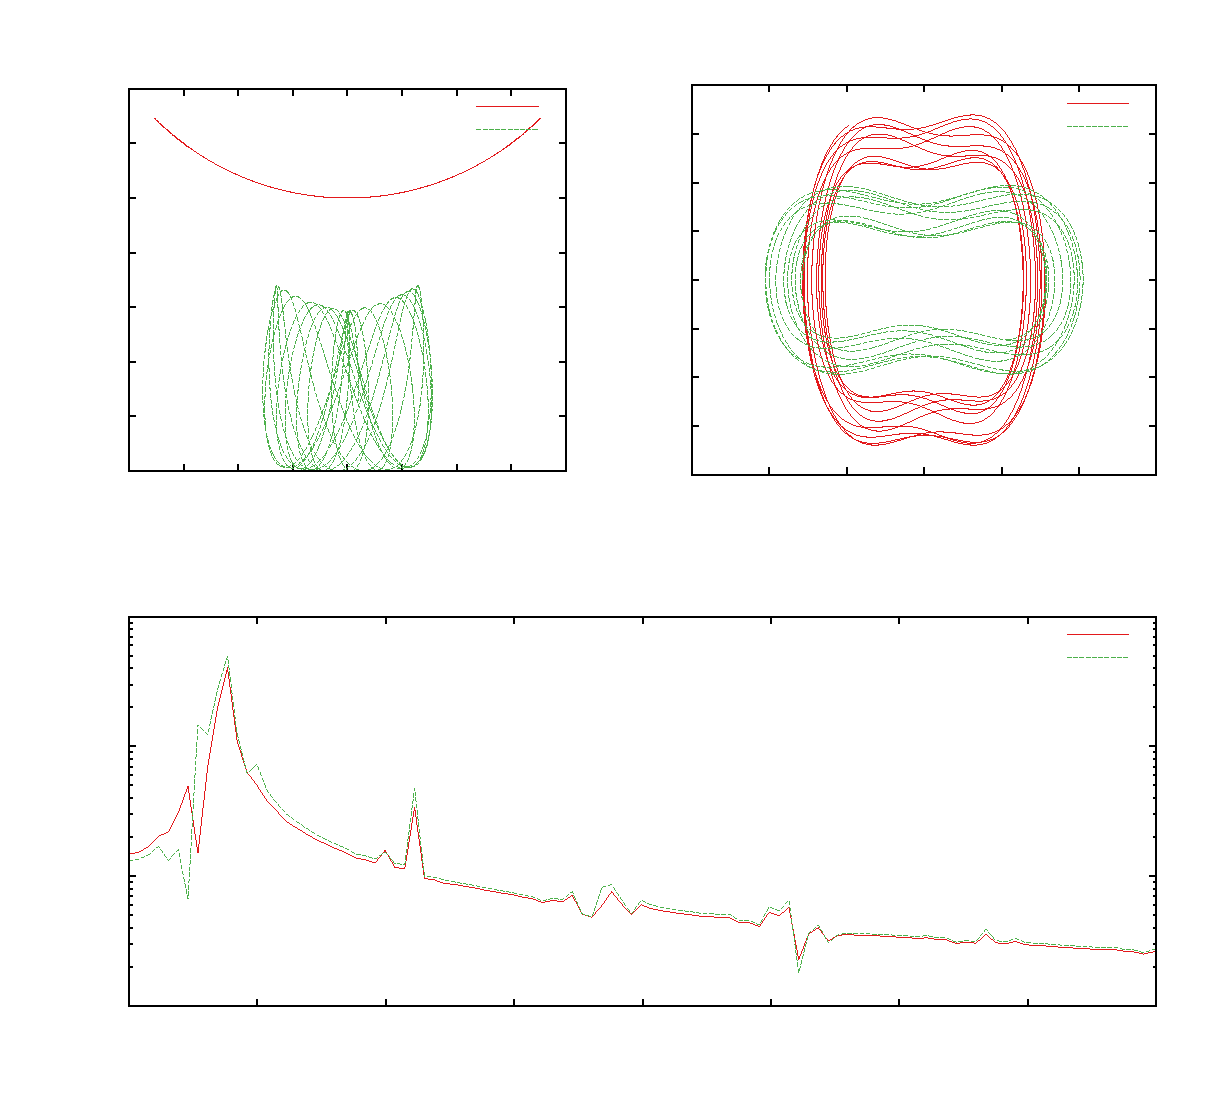
\includegraphics{./figures/trajektorie5}}%
    \gplfronttext
  \end{picture}%
\endgroup
